\section{Gradient Descent and Backpropagation}
\begin{itemize}
	\item Last lecture, we visited the logistic regression, talked about the softmax
		function, and also looked at the log-likelihood loss for gradient descent.
		We were also able to interpret the gradient \(
		\nabla_{\theta}\mathcal{L}(\theta) \) geometrically in terms of how we update
		parameters. 
	\item The gradient is written as:
		\[
			\nabla_{\theta}\mathcal{L}(\theta) = (p_z - y) \nabla_{\theta}z 
		\]
		we write \( p_z - y \) as the "error" term -- so if we were to make an
		incorrect classification, then we would have a nonzero loss.  
\end{itemize}
\subsection{Single-Layer Neural Networks}
\begin{itemize}
	\item As a single layer, we can represent the neural network as follows:
		\begin{center}
			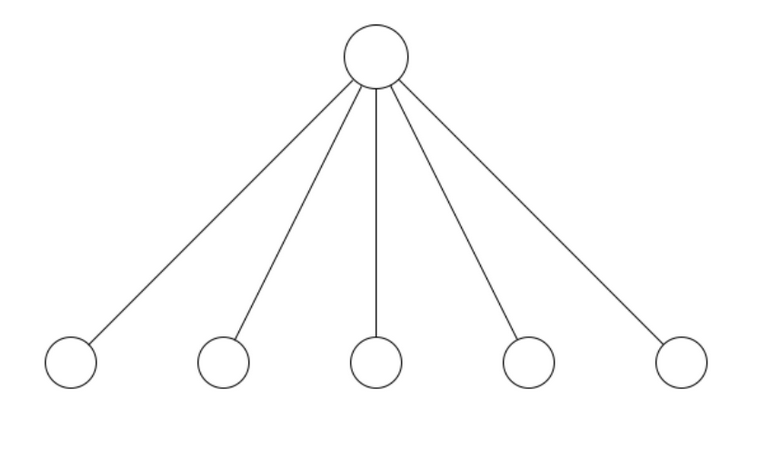
\includegraphics[scale=0.6]{images/one-layer-NN.png}
		\end{center}
		The bottom layer is the input \( x^{(0)} \in \R^{d}\), and the top layer is 
		the output \( x^{(1)} \). Along each "edge" between \( x_i^{(0)} \) and \(
		x^{(1)} \), there are weights \( \theta_{ji} \) which we multiply by their
		respective \( x_i^{(0)} \) to get their contribution in \( x^{(1)} \). 
		So, to calcualte \( x^{(1)} \), we have:
		\[
			x^{(1)} = g\left( \sum_{i} \theta_{ji}^{(1)}x_i^{(0)} \right)
		\]
		\( g(z) \) is called the \textit{activation function}. 
		There are many different values of \( g(z) \) that you can choose: you can
		use a sigmoid, a linear function, or like \( \max(z, 0) \). This last one is
		called ReLU. Another fun one is \( g(z) = \frac{z}{1 + e^{-z}} \), and is
		called SiLU. 
\end{itemize}
\subsection{Two-Layer Neural Networks}
\begin{itemize}
	\item As their name describes, this is the case where you have two layers:
		\begin{center}
			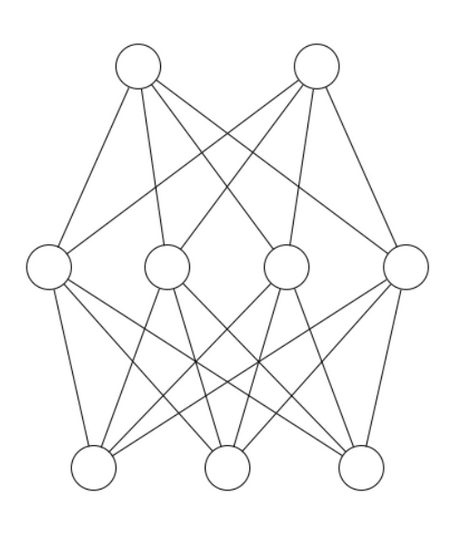
\includegraphics[scale=0.6]{images/two-layer-NN.png}
		\end{center}
		with the following functions:
		\begin{align*}
			x_k^{(2)} = g\left( \sum_j \theta_{kj}^{(2)} x_{j}^{(1)} \right)\\
			x_{j}^{(1)} = g\left( \sum \theta_{ji}^{(0)} x_i^{(0)} \right)
		\end{align*}
		basically, we dot each \( x_j^{(m)} \) with \( \theta_{kj} \) to get \(
		x_k^{(m + 1)} \), then apply the activation function to get the result of the
		next layer. 
	\item In general, each layer has an arbitrary number of layers, so the first
		layer has dimension \( d_0 \) and the second layer \( d_1 \), etc.. You also
		can change \( g \) at every layer, but because this is usually hard to track
		people just stick to a single value of \( g \). 
	\item We also add a unit node that is set to 1 on each layer, which is connected
		to every node in the next layer. This is called the \textit{bias}. 

		\question{why do we introduce the bias?} 

		\answer{We introduce the bias for the same reason we do it in linear
			regression -- we don't want to necessarily restrict the neural network at
			each layer to \textit{have to} pass through \( (0, 0) \), so the bias
		corrects for that.}
	\item We can then generalize this and make our neural net as complicated as we
		want, with the only restriction being that we don't allow any loops. 
	\item As an aside, if you have a function \( f: \R^{d_1} \to \R^{d_2} \), this
		architecture that we've built is actually enough to approximate \( f \) to
		arbitrary accuracy. 
	\item The last layer is also something that is given to us by the problem. If
		we're doing regression which is given by a real value, then the last layer is
		a single node. If we're doing \( K \) classification, then the last layer
		will have dimension \( K \). 
\end{itemize}
\subsection{Gradient Descent}
\begin{itemize}
	\item Before we go any further, we will prove a theorem first:

		\begin{theorem}
			The gradient \( \nabla f(\theta) \) of a function 
			\( f : \Theta \to \R \) at any point \( \theta \) is perpendicular to the
			level set of \( f \) at that point. 
		\end{theorem}

		\begin{proof}
			We define a path \( t \) on the level set in question. Because
			it is a level set, then we know that the level set has the property that
			\( f \) is constant over that set. Thus, for any path \(
			\theta(t) \) we define over the level set, we will have \( \partial_t
			f(\theta(t)) = 0 \). Expanding this:
			\[
				0 = \partial_t f(\theta(t)) 
				= \pdv{f}{\theta_1} \pdv{\theta_1}{t} + \dots
				\pdv{f}{\theta_m} \pdv{\theta_m}{t} = (\nabla f)\cdot \vec v 
			\]
			so, we can only have that \( \vec v \) (or the tangent to the path over
			the level set) is perpendicular to \( \nabla f \), as desired.   
		\end{proof}
	\item Now, consider \( f(\theta) = \frac{\theta^2}{2\alpha} \). This is a
		parabola, where \( \alpha \) controls the "flatness" of the parabola:
		\begin{center}
			\begin{tikzpicture}[domain=-2:2, samples=100]
				\draw[color=blue] plot (\x, {(\x)^2/2}) node[above right]
					{\( \alpha = 1\)} ;
				\draw[color=black] plot (\x, {(\x)^2/8});
				\draw[color=black] plot (\x, {(\x)^2});
				\draw (-5, 0) -- (5, 0);
				\draw (0, -1) -- (0, 5);
			\end{tikzpicture}
		\end{center}
		We ask the question, what does gradient descent look like here?\footnote{As a
		reminder, gradient descent is just a way to "walk along the curve".} Based on
		the rule of gradient descent, we have:
		\[
			\theta_{t + 1} = \theta_t - \epsilon \nabla f(\theta) = \theta_t -
			\epsilon \frac{\theta_t}{\alpha} = \left( 1 - \frac{\epsilon}{\alpha}
			\right) \theta_t
		\]
		Now, suppose you started with some \( \theta_1 \), and we ran this \( t \)
		times. The closed form of \( \theta_t \) is:
		\[
			\theta_t = \left( 1 - \frac{\epsilon}{\alpha} \right)^{t} \theta_1
		\]
		If \( \epsilon < \alpha \), then \( \theta_t \) decreases and approaches zero. 
		If \( \epsilon > \alpha \), then \( \theta_t \) increases, and eventually
		diverges. If \( \epsilon = \alpha \), then after a single step, 
		we've already reached the minimum value so \( \theta_2 = \theta_{min} \). 
	\item So, hopefully this analysis gives some intuition on how the size of 
		\( \epsilon \) that we choose is dependent on \( \alpha \). If \( \alpha \)
		is small, then we likewise need to choose a small \( \epsilon \) in order to
		prevent our function from diverging. 

		Now imagine this in higher dimensions, where the curvature of your level set
		varies depending on where you are on the level set. Then, the \( \epsilon \)
		you choose is constrained by the smallest value of \( \alpha \) that exists
		in the shape.  
\end{itemize}
\subsection{Stochastic Gradient Descent}
\begin{itemize}
	\item Now we will talk about stochastic gradient descent. Here, we will consider
		a loss function, which is expressed as the sum of individual losses:
		\[
			\mathcal{L}(\theta) = \sum_{i = 1}^{n} \mathcal{L}_i(\theta)
		\]
		where \( \mathcal{L}_i(\theta) \) is the loss for any particular data point:
		\[
			\mathcal{L}_i(\theta) = \mathcal{L}(x_i, y_i, \theta)
		\]
		The reason it takes this form is because of the i.i.d. assumption, so that
		when we compute the loss it just ends up being a sum over the loss of an
		individual point. Then, it follows that:
		\[
			L_{i}(\theta) = - \log p_{\theta}(x_i, y_i)
		\]
	\item So far, we've seen two methods to solve this:
		\begin{itemize}
			\item Linear regression:
				\[
					-\log p_{\theta}(x_i, y_i) = \frac{1}{2 \sigma^2} (y_i -
					\theta^{\top} x_i^{(0)} + \text{const.}
				\]
				\question{why do you have a \( \frac{1}{2\sigma^2} \) term here?}

				\answer{The exponent in the Gaussian has a \( \frac{1}{2\sigma^2} \)
				term.} 
			\item Logistic Regression:
				\[
					-\log p_{\theta}(x_i, y_i) = -y_i \log g(\theta^{\top} x_i^{(0)})
					- (1 - y_i) \log(1 - g(\theta^{\top} x_i^{(0)})) + \text{const.}
				\]
		\end{itemize}
	\item Stochastic gradient descent is a process in which you use one of these
		regression losses, and perform the following update scheme:
		\[
			\theta_{t + 1} = \theta_t - \epsilon_t \nabla_{\theta}\mathcal{L}(x_i,
			y_i, \theta)
		\]
		Here, \( \epsilon_t \) is chosen at random, typically without replacement.
		In essence, we are picking at random how large our \( \epsilon \) is.  
	\item This approach has worked in practice -- we usually see that in high
		dimensions the loss is "dominated" by saddle points (so false minima), and
		the variance introduced by SGD seems to avoid these points. 

		That said, it has also been shown that the noise hurts us when we get close
		to the optimal point, slowing the algorithm down. There is a compromise that
		you can make, which is to divide the dataset into \( b \) batches of size \(
		n / b\), where for each batch you compute the loss and perform the
		corresponding update.  
\end{itemize}
